\documentclass[border=0in]{standalone}
\usepackage{tikz}
\usepackage{xcolor}
\usepackage{array}
\usetikzlibrary{shapes.misc, patterns}

\begin{document}
%%%%%%%%%%%%%%%%%%%%%%%%%%%%%%%%%%%%%%%%%%%%%%%%%%
%%%%%%%%%%%%%%%%%%%%%%%%%%%%%%%%%%%%%%%%%%%%%%%%%%
\begin{tabular}{ c  c  c  c }

% Expt EV
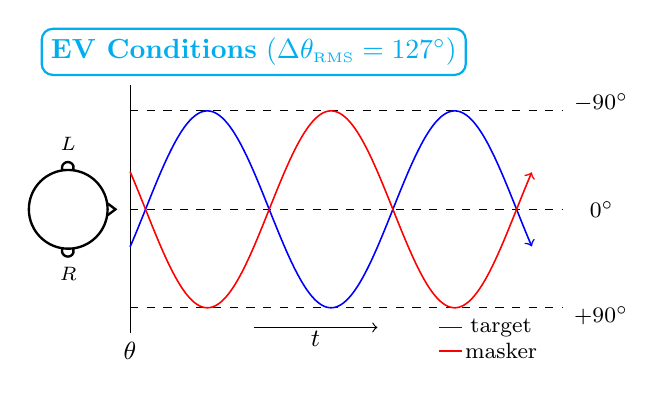
\begin{tikzpicture}
  % Title
  \node[draw=cyan, text=cyan, thick, rounded corners, opacity=1] at (3*pi/4, 2) {\textbf{EV Conditions} ($\Delta \theta_{\textrm{\tiny RMS}} = 127^{\circ}$)};
  
  % Legend
  \draw[line width=0.2mm, blue] (3*pi/2, -1.5) -- (3*pi/2 + 3*pi/32, -1.5);
  \node at (3*pi/2 + 8*pi/32, -1.5) {\footnotesize target};
  \draw[line width=0.2mm,  red] (3*pi/2, -1.8) -- (3*pi/2 + 3*pi/32, -1.8);
  \node at (3*pi/2 + 8*pi/32, -1.8) {\footnotesize masker};
  
  % y axis
  \draw[line width=0.125mm, black] (pi/4, -1.575) -- (pi/4, 1.575);
  \node at (pi/4, -1.8) {\small $\theta$};
  
  % Dashed degree guide lines
  \draw[line width=0.125mm, black, dashed] (pi/4,  1.25) -- (2*pi,  1.25);
  \draw[line width=0.125mm, black, dashed] (pi/4,  0.)   -- (2*pi,  0.  );
  \draw[line width=0.125mm, black, dashed] (pi/4, -1.25) -- (2*pi, -1.25);
  
  % Degree guides
  \node[align=right, text width=0.5cm] at (2*pi + pi/8,  1.35)
    {\footnotesize $-90^{\circ}$};
  \node[align=right, text width=0.5cm] at (2*pi + pi/8,  0.)
    {\footnotesize $0^{\circ}$};
  \node[align=right, text width=0.5cm] at (2*pi + pi/8, -1.35)
    {\footnotesize $+90^{\circ}$};
  
  % Arrow of time
  \draw[help lines, ->, line width=0.15mm, black] (3*pi/4, -1.5) -- (5*pi/4, -1.5);
  \node at (pi, -1.65) {\small $t$};
  
  % Sinusoids
  \draw[help lines, ->, line width=0.2mm, blue, domain=pi/4:2*pi - pi/8, samples=1000]
        plot(\x, {-1.25*sin((2*\x + 3*pi/8) r)});
  \draw[help lines, ->, line width=0.2mm,  red, domain=pi/4:2*pi - pi/8, samples=1000]
        plot(\x, { 1.25*sin((2*\x + 3*pi/8) r)});
  
  % Head
  \node at (0, 0.825) {\scriptsize $L$};
  \draw[line width=0.3mm] (0, 0) circle (0.5cm); % head
  \draw[line width=0.3mm] (0 - 0.075,  0.5) arc ( 200:-20:0.075); % R ear
  \draw[line width=0.3mm]
         (0 + 0.5,  0.075) --
         (0 + 0.6,  0.   ) --
         (0 + 0.5, -0.075); % nose
  \draw[line width=0.3mm] (0 - 0.075, -0.5) arc (-200: 20:0.075); % L ear
  \node at (0, -0.825) {\scriptsize $R$};
\end{tikzpicture}


&


%%% Expt EV stim conditions
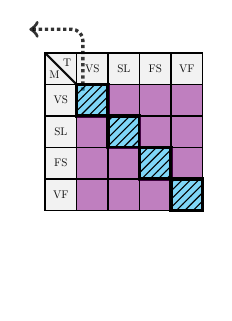
\begin{tikzpicture}[scale=0.4, every node/.style={transform shape}]
  % Target/Masker
  \node at (0.7, 6.2) {T};
  \node at (0.3, 5.8) {M};
  \draw[thick] (0, 6.5) -- (1, 5.5);
  
  % Row labels
  \node at (1.5, 6.) {VS};
  \node at (2.5, 6.) {SL};
  \node at (3.5, 6.) {FS};
  \node at (4.5, 6.) {VF};
  % Column labels
  \node at (0.5, 5.) {VS};
  \node at (0.5, 4.) {SL};
  \node at (0.5, 3.) {FS};
  \node at (0.5, 2.) {VF};
  
  % Row 1 (top)
  \draw[help lines, ->, black, very thick, densely dotted, opacity=0.8, rounded corners] (1.2, 5.3) -- (1.2, 7.25) -- (-0.5, 7.25);
  \draw[semithick, draw=black, fill=gray, fill opacity=0.1]
     (0, 5.5) -- (0, 6.5) -- (1, 6.5) -- (1, 5.5) -- cycle;
  \draw[semithick, draw=black, fill=gray, fill opacity=0.1]
     (1, 5.5) -- (1, 6.5) -- (2, 6.5) -- (2, 5.5) -- cycle;
  \draw[semithick, draw=black, fill=gray, fill opacity=0.1]
     (2, 5.5) -- (2, 6.5) -- (3, 6.5) -- (3, 5.5) -- cycle;
  \draw[semithick, draw=black, fill=gray, fill opacity=0.1]
     (3, 5.5) -- (3, 6.5) -- (4, 6.5) -- (4, 5.5) -- cycle;
  \draw[semithick, draw=black, fill=gray, fill opacity=0.1]
     (4, 5.5) -- (4, 6.5) -- (5, 6.5) -- (5, 5.5) -- cycle;
  % Row 2
  \draw[semithick, draw=black, fill=gray, fill opacity=0.1]
     (0, 4.5) -- (0, 5.5) -- (1, 5.5) -- (1, 4.5) -- cycle;
  \draw[very thick, draw=black, fill=cyan, fill opacity=0.5]
     (1, 4.5) -- (1, 5.5) -- (2, 5.5) -- (2, 4.5) -- cycle;
  \draw[semithick, draw=black, pattern=north east lines]
     (1, 4.5) -- (1, 5.5) -- (2, 5.5) -- (2, 4.5) -- cycle;
  \draw[semithick, draw=black, fill=violet, fill opacity=0.5]
     (2, 4.5) -- (2, 5.5) -- (3, 5.5) -- (3, 4.5) -- cycle;
  \draw[semithick, draw=black, fill=violet, fill opacity=0.5]
     (3, 4.5) -- (3, 5.5) -- (4, 5.5) -- (4, 4.5) -- cycle;
  \draw[semithick, draw=black, fill=violet, fill opacity=0.5]
     (4, 4.5) -- (4, 5.5) -- (5, 5.5) -- (5, 4.5) -- cycle;
  % Row 3
  \draw[semithick, draw=black, fill=gray, fill opacity=0.1]
     (0, 3.5) -- (0, 4.5) -- (1, 4.5) -- (1, 3.5) -- cycle;
  \draw[semithick, draw=black, fill=violet, fill opacity=0.5]
     (1, 3.5) -- (1, 4.5) -- (2, 4.5) -- (2, 3.5) -- cycle;
  \draw[very thick, draw=black, fill=cyan, fill opacity=0.5]
     (2, 3.5) -- (2, 4.5) -- (3, 4.5) -- (3, 3.5) -- cycle;
  \draw[semithick, draw=black, pattern=north east lines]
     (2, 3.5) -- (2, 4.5) -- (3, 4.5) -- (3, 3.5) -- cycle;
  \draw[semithick, draw=black, fill=violet, fill opacity=0.5]
     (3, 3.5) -- (3, 4.5) -- (4, 4.5) -- (4, 3.5) -- cycle;
  \draw[semithick, draw=black, fill=violet, fill opacity=0.5]
     (4, 3.5) -- (4, 4.5) -- (5, 4.5) -- (5, 3.5) -- cycle;
  % Row 4
  \draw[semithick, draw=black, fill=gray, fill opacity=0.1]
     (0, 2.5) -- (0, 3.5) -- (1, 3.5) -- (1, 2.5) -- cycle;
  \draw[semithick, draw=black, fill=violet, fill opacity=0.5]
     (1, 2.5) -- (1, 3.5) -- (2, 3.5) -- (2, 2.5) -- cycle;
  \draw[semithick, draw=black, fill=violet, fill opacity=0.5]
     (2, 2.5) -- (2, 3.5) -- (3, 3.5) -- (3, 2.5) -- cycle;
  \draw[very thick, draw=black, fill=cyan, fill opacity=0.5]
     (3, 2.5) -- (3, 3.5) -- (4, 3.5) -- (4, 2.5) -- cycle;
  \draw[semithick, draw=black, pattern=north east lines]
     (3, 2.5) -- (3, 3.5) -- (4, 3.5) -- (4, 2.5) -- cycle;
  \draw[semithick, draw=black, fill=violet, fill opacity=0.5]
     (4, 2.5) -- (4, 3.5) -- (5, 3.5) -- (5, 2.5) -- cycle;
  % Row 5 (bottom)
  \draw[semithick, draw=black, fill=gray, fill opacity=0.1]
     (0, 1.5) -- (0, 2.5) -- (1, 2.5) -- (1, 1.5) -- cycle;
  \draw[semithick, draw=black, fill=violet, fill opacity=0.5]
     (1, 1.5) -- (1, 2.5) -- (2, 2.5) -- (2, 1.5) -- cycle;
  \draw[semithick, draw=black, fill=violet, fill opacity=0.5]
     (2, 1.5) -- (2, 2.5) -- (3, 2.5) -- (3, 1.5) -- cycle;
  \draw[semithick, draw=black, fill=violet, fill opacity=0.5]
     (3, 1.5) -- (3, 2.5) -- (4, 2.5) -- (4, 1.5) -- cycle;
  \draw[very thick, draw=black, fill=cyan, fill opacity=0.5]
     (4, 1.5) -- (4, 2.5) -- (5, 2.5) -- (5, 1.5) -- cycle;
  \draw[semithick, draw=black, pattern=north east lines]
     (4, 1.5) -- (4, 2.5) -- (5, 2.5) -- (5, 1.5) -- cycle;

  % Invisible node to force the matrix up
  \node at (0, -1) {};
\end{tikzpicture}


&


%%% Hypothesis 1
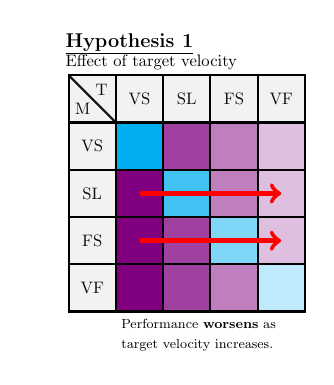
\begin{tikzpicture}[scale=0.6, every node/.style={transform shape}]
  % Prediction label
  \node[align=left] at (1.75, 5.5) {\large\underline{\textbf{Hypothesis 1}}\\Effect of target velocity};
  %\node at (1.8, 5.35) {\small Effect of target velocity};
  %\node[draw, very thick, rounded corners] at (1.4, 5.9) {\large\textbf{Hypothesis 1}};
  %\node at (1.8, 5.35) {\small Effect of target velocity};

  % Target/Masker
  \node at (0.7, 4.7) {T};
  \node at (0.3, 4.3) {M};
  \draw[thick] (0, 5) -- (1, 4);
  
  % Row labels
  \node at (1.5, 4.5) {VS};
  \node at (2.5, 4.5) {SL};
  \node at (3.5, 4.5) {FS};
  \node at (4.5, 4.5) {VF};
  % Column labels
  \node at (0.5, 3.5) {VS};
  \node at (0.5, 2.5) {SL};
  \node at (0.5, 1.5) {FS};
  \node at (0.5, 0.5) {VF};
  
  % Row 1 (top)
  \draw[thick, draw=black, fill=gray, fill opacity=0.1]
     (0, 4) -- (0, 5) -- (1, 5) -- (1, 4) -- cycle;
  \draw[thick, draw=black, fill=gray, fill opacity=0.1]
     (1, 4) -- (1, 5) -- (2, 5) -- (2, 4) -- cycle;
  \draw[thick, draw=black, fill=gray, fill opacity=0.1]
     (2, 4) -- (2, 5) -- (3, 5) -- (3, 4) -- cycle;
  \draw[thick, draw=black, fill=gray, fill opacity=0.1]
     (3, 4) -- (3, 5) -- (4, 5) -- (4, 4) -- cycle;
  \draw[thick, draw=black, fill=gray, fill opacity=0.1]
     (4, 4) -- (4, 5) -- (5, 5) -- (5, 4) -- cycle;
  % Row 2
  \draw[thick, draw=black, fill=gray, fill opacity=0.1]
     (0, 3) -- (0, 4) -- (1, 4) -- (1, 3) -- cycle;
  \draw[thick, draw=black, fill=cyan, fill opacity=1.]
     (1, 3) -- (1, 4) -- (2, 4) -- (2, 3) -- cycle;
  \draw[thick, draw=black, fill=violet, fill opacity=0.75]
     (2, 3) -- (2, 4) -- (3, 4) -- (3, 3) -- cycle;
  \draw[thick, draw=black, fill=violet, fill opacity=0.5]
     (3, 3) -- (3, 4) -- (4, 4) -- (4, 3) -- cycle;
  \draw[thick, draw=black, fill=violet, fill opacity=0.25]
     (4, 3) -- (4, 4) -- (5, 4) -- (5, 3) -- cycle;
  % Row 3
  \draw[thick, draw=black, fill=gray, fill opacity=0.1]
     (0, 2) -- (0, 3) -- (1, 3) -- (1, 2) -- cycle;
  \draw[thick, draw=black, fill=violet, fill opacity=1.]
     (1, 2) -- (1, 3) -- (2, 3) -- (2, 2) -- cycle;
  \draw[thick, draw=black, fill=cyan, fill opacity=0.75]
     (2, 2) -- (2, 3) -- (3, 3) -- (3, 2) -- cycle;
  \draw[thick, draw=black, fill=violet, fill opacity=0.5]
     (3, 2) -- (3, 3) -- (4, 3) -- (4, 2) -- cycle;
  \draw[thick, draw=black, fill=violet, fill opacity=0.25]
     (4, 2) -- (4, 3) -- (5, 3) -- (5, 2) -- cycle;
  % Row 4
  \draw[thick, draw=black, fill=gray, fill opacity=0.1]
     (0, 1) -- (0, 2) -- (1, 2) -- (1, 1) -- cycle;
  \draw[thick, draw=black, fill=violet, fill opacity=1.]
     (1, 1) -- (1, 2) -- (2, 2) -- (2, 1) -- cycle;
  \draw[thick, draw=black, fill=violet, fill opacity=0.75]
     (2, 1) -- (2, 2) -- (3, 2) -- (3, 1) -- cycle;
  \draw[thick, draw=black, fill=cyan, fill opacity=0.5]
     (3, 1) -- (3, 2) -- (4, 2) -- (4, 1) -- cycle;
  \draw[thick, draw=black, fill=violet, fill opacity=0.25]
     (4, 1) -- (4, 2) -- (5, 2) -- (5, 1) -- cycle;
  % Row 5 (bottom)
  \draw[thick, draw=black, fill=gray, fill opacity=0.1]
     (0, 0) -- (0, 1) -- (1, 1) -- (1, 0) -- cycle;
  \draw[thick, draw=black, fill=violet, fill opacity=1.]
     (1, 0) -- (1, 1) -- (2, 1) -- (2, 0) -- cycle;
  \draw[thick, draw=black, fill=violet, fill opacity=0.75]
     (2, 0) -- (2, 1) -- (3, 1) -- (3, 0) -- cycle;
  \draw[thick, draw=black, fill=violet, fill opacity=0.5]
     (3, 0) -- (3, 1) -- (4, 1) -- (4, 0) -- cycle;
  \draw[thick, draw=black, fill=cyan, fill opacity=0.25]
     (4, 0) -- (4, 1) -- (5, 1) -- (5, 0) -- cycle;
  
  % Prediction help
  \draw[help lines, ->, red, ultra thick] (1.5, 2.5) -- (4.5, 2.5);
  \draw[help lines, ->, red, ultra thick] (1.5, 1.5) -- (4.5, 1.5);
  \node[align=left] at (2.75, -0.5) {\footnotesize Performance \textbf{worsens} as\\\footnotesize target velocity increases.};

  % Invisible node to force the matrix up
  \node at (-0.75, 0) {};
\end{tikzpicture}


&


%%% Hypothesis 2
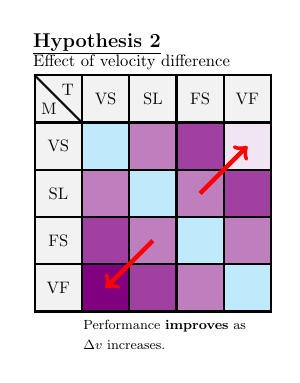
\begin{tikzpicture}[scale=0.6, every node/.style={transform shape}]
  % Prediction label
  \node[align=left] at (2.05, 5.5) {\large\underline{\textbf{Hypothesis 2}}\\Effect of velocity difference};
  %\node[draw, very thick, rounded corners] at (1.4, 5.9) {\large\textbf{Hypothesis 2}};
  %\node at (2.075, 5.35) {\small Effect of velocity difference};
  
  % Target/Masker
  \node at (0.7, 4.7) {T};
  \node at (0.3, 4.3) {M};
  \draw[thick] (0, 5) -- (1, 4);
  
  % Row labels
  \node at (1.5, 4.5) {VS};
  \node at (2.5, 4.5) {SL};
  \node at (3.5, 4.5) {FS};
  \node at (4.5, 4.5) {VF};
  % Column labels
  \node at (0.5, 3.5) {VS};
  \node at (0.5, 2.5) {SL};
  \node at (0.5, 1.5) {FS};
  \node at (0.5, 0.5) {VF};
  
  % Row 1 (top)
  \draw[thick, draw=black, fill=gray, fill opacity=0.1]
     (0, 4) -- (0, 5) -- (1, 5) -- (1, 4) -- cycle;
  \draw[thick, draw=black, fill=gray, fill opacity=0.1]
     (1, 4) -- (1, 5) -- (2, 5) -- (2, 4) -- cycle;
  \draw[thick, draw=black, fill=gray, fill opacity=0.1]
     (2, 4) -- (2, 5) -- (3, 5) -- (3, 4) -- cycle;
  \draw[thick, draw=black, fill=gray, fill opacity=0.1]
     (3, 4) -- (3, 5) -- (4, 5) -- (4, 4) -- cycle;
  \draw[thick, draw=black, fill=gray, fill opacity=0.1]
     (4, 4) -- (4, 5) -- (5, 5) -- (5, 4) -- cycle;
  % Row 2
  \draw[thick, draw=black, fill=gray, fill opacity=0.1]
     (0, 3) -- (0, 4) -- (1, 4) -- (1, 3) -- cycle;
  \draw[thick, draw=black, fill=cyan, fill opacity=0.25]
     (1, 3) -- (1, 4) -- (2, 4) -- (2, 3) -- cycle;
  \draw[thick, draw=black, fill=violet, fill opacity=0.5]
     (2, 3) -- (2, 4) -- (3, 4) -- (3, 3) -- cycle;
  \draw[thick, draw=black, fill=violet, fill opacity=0.75]
     (3, 3) -- (3, 4) -- (4, 4) -- (4, 3) -- cycle;
  \draw[thick, draw=black, fill=violet, fill opacity=0.1.]
     (4, 3) -- (4, 4) -- (5, 4) -- (5, 3) -- cycle;
  % Row 3
  \draw[thick, draw=black, fill=gray, fill opacity=0.1]
     (0, 2) -- (0, 3) -- (1, 3) -- (1, 2) -- cycle;
  \draw[thick, draw=black, fill=violet, fill opacity=0.5]
     (1, 2) -- (1, 3) -- (2, 3) -- (2, 2) -- cycle;
  \draw[thick, draw=black, fill=cyan, fill opacity=0.25]
     (2, 2) -- (2, 3) -- (3, 3) -- (3, 2) -- cycle;
  \draw[thick, draw=black, fill=violet, fill opacity=0.5]
     (3, 2) -- (3, 3) -- (4, 3) -- (4, 2) -- cycle;
  \draw[thick, draw=black, fill=violet, fill opacity=0.75]
     (4, 2) -- (4, 3) -- (5, 3) -- (5, 2) -- cycle;
  % Row 4
  \draw[thick, draw=black, fill=gray, fill opacity=0.1]
     (0, 1) -- (0, 2) -- (1, 2) -- (1, 1) -- cycle;
  \draw[thick, draw=black, fill=violet, fill opacity=0.75]
     (1, 1) -- (1, 2) -- (2, 2) -- (2, 1) -- cycle;
  \draw[thick, draw=black, fill=violet, fill opacity=0.5]
     (2, 1) -- (2, 2) -- (3, 2) -- (3, 1) -- cycle;
  \draw[thick, draw=black, fill=cyan, fill opacity=0.25]
     (3, 1) -- (3, 2) -- (4, 2) -- (4, 1) -- cycle;
  \draw[thick, draw=black, fill=violet, fill opacity=0.5]
     (4, 1) -- (4, 2) -- (5, 2) -- (5, 1) -- cycle;
  % Row 5 (bottom)
  \draw[thick, draw=black, fill=gray, fill opacity=0.1]
     (0, 0) -- (0, 1) -- (1, 1) -- (1, 0) -- cycle;
  \draw[thick, draw=black, fill=violet, fill opacity=1.]
     (1, 0) -- (1, 1) -- (2, 1) -- (2, 0) -- cycle;
  \draw[thick, draw=black, fill=violet, fill opacity=0.75]
     (2, 0) -- (2, 1) -- (3, 1) -- (3, 0) -- cycle;
  \draw[thick, draw=black, fill=violet, fill opacity=0.5]
     (3, 0) -- (3, 1) -- (4, 1) -- (4, 0) -- cycle;
  \draw[thick, draw=black, fill=cyan, fill opacity=0.25]
     (4, 0) -- (4, 1) -- (5, 1) -- (5, 0) -- cycle;
  
  % Prediction help
  \draw[help lines, <-, red, ultra thick] (1.5, 0.5) -- (2.5, 1.5);
  \draw[help lines, ->, red, ultra thick] (3.5, 2.5) -- (4.5, 3.5);
  \node[align=left] at (2.75, -0.5) {\footnotesize Performance \textbf{improves} as\\\footnotesize $\Delta v$ increases.};
\end{tikzpicture}



\vspace{0.25 in}
\\
\vspace{0.25 in}



% Expt DV
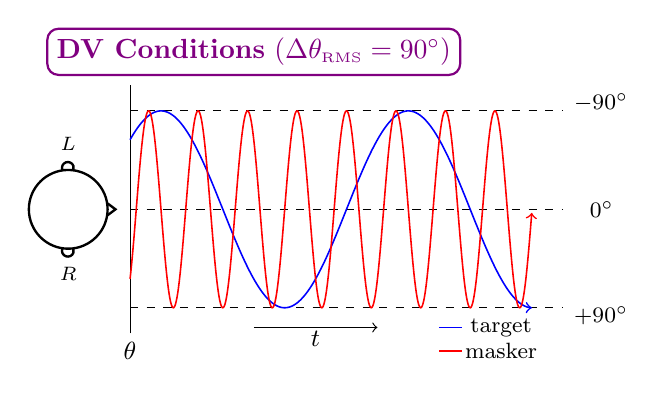
\begin{tikzpicture}
  % Title
  \node[draw=violet, text=violet, thick, rounded corners, opacity=1] at (3*pi/4, 2) {\textbf{DV Conditions} ($\Delta \theta_{\textrm{\tiny RMS}} = 90^{\circ}$)};
  
  % Legend
  \draw[line width=0.2mm, blue] (3*pi/2, -1.5) -- (3*pi/2 + 3*pi/32, -1.5);
  \node at (3*pi/2 + 8*pi/32, -1.5) {\footnotesize target};
  \draw[line width=0.2mm,  red] (3*pi/2, -1.8) -- (3*pi/2 + 3*pi/32, -1.8);
  \node at (3*pi/2 + 8*pi/32, -1.8) {\footnotesize masker};
  
  % y axis
  \draw[line width=0.125mm, black] (pi/4, -1.575) -- (pi/4, 1.575);
  \node at (pi/4, -1.8) {\small $\theta$};
  
  % Dashed degree guide lines
  \draw[line width=0.125mm, black, dashed] (pi/4,  1.25) -- (2*pi,  1.25);
  \draw[line width=0.125mm, black, dashed] (pi/4,  0.)   -- (2*pi,  0.  );
  \draw[line width=0.125mm, black, dashed] (pi/4, -1.25) -- (2*pi, -1.25);
  
  % Degree guides
  \node[align=right, text width=0.5cm] at (2*pi + pi/8,  1.35)
    {\footnotesize $-90^{\circ}$};
  \node[align=right, text width=0.5cm] at (2*pi + pi/8,  0.)
    {\footnotesize $0^{\circ}$};
  \node[align=right, text width=0.5cm] at (2*pi + pi/8, -1.35)
    {\footnotesize $+90^{\circ}$};
  
  % Arrow of time
  \draw[help lines, ->, line width=0.15mm, black] (3*pi/4, -1.5) -- (5*pi/4, -1.5);
  \node at (pi, -1.65) {\small $t$};
  
  % Sinusoids
  \draw[help lines, ->, line width=0.2mm, blue, domain=pi/4:2*pi - pi/8, samples=1000]
        plot(\x, {1.25*sin(( 2*\x - pi/4) r)});
  \draw[help lines, ->, line width=0.2mm,  red, domain=pi/4:2*pi - pi/8, samples=1000]
        plot(\x, {1.25*sin((10*\x - 3*pi/4) r)});
   
  % Head
  \node at (0, 0.825) {\scriptsize $L$};
  \draw[line width=0.3mm] (0, 0) circle (0.5cm); % head
  \draw[line width=0.3mm] (0 - 0.075,  0.5) arc ( 200:-20:0.075); % R ear
  \draw[line width=0.3mm]
         (0 + 0.5,  0.075) --
         (0 + 0.6,  0.   ) --
         (0 + 0.5, -0.075); % nose
  \draw[line width=0.3mm] (0 - 0.075, -0.5) arc (-200: 20:0.075); % L ear
  \node at (0, -0.825) {\scriptsize $R$};
\end{tikzpicture}


&


%%% Expt DV stim conditions
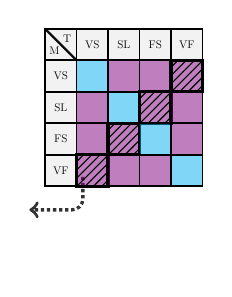
\begin{tikzpicture}[scale=0.4, every node/.style={transform shape}]
  % Target/Masker
  \node at (0.7, 6.2) {T};
  \node at (0.3, 5.8) {M};
  \draw[thick] (0, 6.5) -- (1, 5.5);
  
  % Row labels
  \node at (1.5, 6.) {VS};
  \node at (2.5, 6.) {SL};
  \node at (3.5, 6.) {FS};
  \node at (4.5, 6.) {VF};
  % Column labels
  \node at (0.5, 5.) {VS};
  \node at (0.5, 4.) {SL};
  \node at (0.5, 3.) {FS};
  \node at (0.5, 2.) {VF};
  
  % Row 1 (top)
  \draw[help lines, ->, black, very thick, densely dotted, opacity=0.8, rounded corners] (1.2, 1.8) -- (1.2, 0.75) -- (-0.5, 0.75);
  \draw[semithick, draw=black, fill=gray, fill opacity=0.1]
     (0, 5.5) -- (0, 6.5) -- (1, 6.5) -- (1, 5.5) -- cycle;
  \draw[semithick, draw=black, fill=gray, fill opacity=0.1]
     (1, 5.5) -- (1, 6.5) -- (2, 6.5) -- (2, 5.5) -- cycle;
  \draw[semithick, draw=black, fill=gray, fill opacity=0.1]
     (2, 5.5) -- (2, 6.5) -- (3, 6.5) -- (3, 5.5) -- cycle;
  \draw[semithick, draw=black, fill=gray, fill opacity=0.1]
     (3, 5.5) -- (3, 6.5) -- (4, 6.5) -- (4, 5.5) -- cycle;
  \draw[semithick, draw=black, fill=gray, fill opacity=0.1]
     (4, 5.5) -- (4, 6.5) -- (5, 6.5) -- (5, 5.5) -- cycle;
  % Row 2
  \draw[semithick, draw=black, fill=gray, fill opacity=0.1]
     (0, 4.5) -- (0, 5.5) -- (1, 5.5) -- (1, 4.5) -- cycle;
  \draw[semithick, draw=black, fill=cyan, fill opacity=0.5]
     (1, 4.5) -- (1, 5.5) -- (2, 5.5) -- (2, 4.5) -- cycle;
  \draw[semithick, draw=black, fill=violet, fill opacity=0.5]
     (2, 4.5) -- (2, 5.5) -- (3, 5.5) -- (3, 4.5) -- cycle;
  \draw[semithick, draw=black, fill=violet, fill opacity=0.5]
     (3, 4.5) -- (3, 5.5) -- (4, 5.5) -- (4, 4.5) -- cycle;
  \draw[very thick, draw=black, fill=violet, fill opacity=0.5]
     (4, 4.5) -- (4, 5.5) -- (5, 5.5) -- (5, 4.5) -- cycle;
  \draw[semithick, draw=black, pattern=north east lines]
     (4, 4.5) -- (4, 5.5) -- (5, 5.5) -- (5, 4.5) -- cycle;
  % Row 3
  \draw[semithick, draw=black, fill=gray, fill opacity=0.1]
     (0, 3.5) -- (0, 4.5) -- (1, 4.5) -- (1, 3.5) -- cycle;
  \draw[semithick, draw=black, fill=violet, fill opacity=0.5]
     (1, 3.5) -- (1, 4.5) -- (2, 4.5) -- (2, 3.5) -- cycle;
  \draw[semithick, draw=black, fill=cyan, fill opacity=0.5]
     (2, 3.5) -- (2, 4.5) -- (3, 4.5) -- (3, 3.5) -- cycle;
  \draw[very thick, draw=black, fill=violet, fill opacity=0.5]
     (3, 3.5) -- (3, 4.5) -- (4, 4.5) -- (4, 3.5) -- cycle;
  \draw[semithick, draw=black, pattern=north east lines]
     (3, 3.5) -- (3, 4.5) -- (4, 4.5) -- (4, 3.5) -- cycle;
  \draw[semithick, draw=black, fill=violet, fill opacity=0.5]
     (4, 3.5) -- (4, 4.5) -- (5, 4.5) -- (5, 3.5) -- cycle;
  % Row 4
  \draw[semithick, draw=black, fill=gray, fill opacity=0.1]
     (0, 2.5) -- (0, 3.5) -- (1, 3.5) -- (1, 2.5) -- cycle;
  \draw[semithick, draw=black, fill=violet, fill opacity=0.5]
     (1, 2.5) -- (1, 3.5) -- (2, 3.5) -- (2, 2.5) -- cycle;
  \draw[very thick, draw=black, fill=violet, fill opacity=0.5]
     (2, 2.5) -- (2, 3.5) -- (3, 3.5) -- (3, 2.5) -- cycle;
  \draw[semithick, draw=black, pattern=north east lines]
     (2, 2.5) -- (2, 3.5) -- (3, 3.5) -- (3, 2.5) -- cycle;
  \draw[semithick, draw=black, fill=cyan, fill opacity=0.5]
     (3, 2.5) -- (3, 3.5) -- (4, 3.5) -- (4, 2.5) -- cycle;
  \draw[semithick, draw=black, fill=violet, fill opacity=0.5]
     (4, 2.5) -- (4, 3.5) -- (5, 3.5) -- (5, 2.5) -- cycle;
  % Row 5 (bottom)
  \draw[semithick, draw=black, fill=gray, fill opacity=0.1]
     (0, 1.5) -- (0, 2.5) -- (1, 2.5) -- (1, 1.5) -- cycle;
  \draw[very thick, draw=black, fill=violet, fill opacity=0.5]
     (1, 1.5) -- (1, 2.5) -- (2, 2.5) -- (2, 1.5) -- cycle;
  \draw[semithick, draw=black, pattern=north east lines]
     (1, 1.5) -- (1, 2.5) -- (2, 2.5) -- (2, 1.5) -- cycle;
  \draw[semithick, draw=black, fill=violet, fill opacity=0.5]
     (2, 1.5) -- (2, 2.5) -- (3, 2.5) -- (3, 1.5) -- cycle;
  \draw[semithick, draw=black, fill=violet, fill opacity=0.5]
     (3, 1.5) -- (3, 2.5) -- (4, 2.5) -- (4, 1.5) -- cycle;
  \draw[semithick, draw=black, fill=cyan, fill opacity=0.5]
     (4, 1.5) -- (4, 2.5) -- (5, 2.5) -- (5, 1.5) -- cycle;

  % Invisible node to force the matrix up
  \node at (0, -1) {};
\end{tikzpicture}


&


%%% EM data
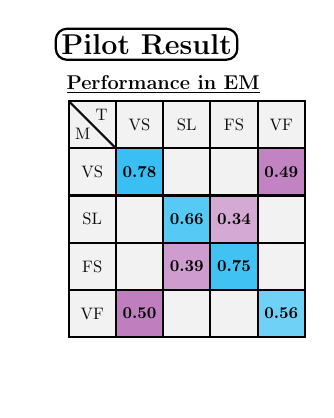
\begin{tikzpicture}[scale=0.6, every node/.style={transform shape}]
  % RESULT
  \node[draw, thick, rounded corners] at (1.65, 12.7) {\LARGE\textbf{Pilot Result}};
  
  % Label
  \node at (2., 11.85) {\large\underline{\textbf{Performance in EM}}};
  
  % Target/Masker
  \node at (0.7, 11.2) {T};
  \node at (0.3, 10.8) {M};
  \draw[thick] (0, 11.5) -- (1, 10.5);
  
  % Row labels
  \node at (1.5, 11.) {VS};
  \node at (2.5, 11.) {SL};
  \node at (3.5, 11.) {FS};
  \node at (4.5, 11.) {VF};
  % Column labels
  \node at (0.5, 10.) {VS};
  \node at (0.5, 9.) {SL};
  \node at (0.5, 8.) {FS};
  \node at (0.5, 7.) {VF};
  
  % Row 1 (top)
  \draw[thick, draw=black, fill=gray, fill opacity=0.1]
     (0, 10.5) -- (0, 11.5) -- (1, 11.5) -- (1, 10.5) -- cycle;
  \draw[thick, draw=black, fill=gray, fill opacity=0.1]
     (1, 10.5) -- (1, 11.5) -- (2, 11.5) -- (2, 10.5) -- cycle;
  \draw[thick, draw=black, fill=gray, fill opacity=0.1]
     (2, 10.5) -- (2, 11.5) -- (3, 11.5) -- (3, 10.5) -- cycle;
  \draw[thick, draw=black, fill=gray, fill opacity=0.1]
     (3, 10.5) -- (3, 11.5) -- (4, 11.5) -- (4, 10.5) -- cycle;
  \draw[thick, draw=black, fill=gray, fill opacity=0.1]
     (4, 10.5) -- (4, 11.5) -- (5, 11.5) -- (5, 10.5) -- cycle;
  % Row 2
  \draw[thick, draw=black, fill=gray, fill opacity=0.1]
     (0, 9.5) -- (0, 10.5) -- (1, 10.5) -- (1, 9.5) -- cycle;
  \draw[thick, draw=black, fill=cyan, fill opacity=0.775]
     (1, 9.5) -- (1, 10.5) -- (2, 10.5) -- (2, 9.5) -- cycle;
  \node at (1.5, 10.) {\textbf{0.78}};
  \draw[thick, draw=black, fill=gray, fill opacity=0.1]
     (2, 9.5) -- (2, 10.5) -- (3, 10.5) -- (3, 9.5) -- cycle;
  \draw[thick, draw=black, fill=gray, fill opacity=0.1]
     (3, 9.5) -- (3, 10.5) -- (4, 10.5) -- (4, 9.5) -- cycle;
  \draw[thick, draw=black, fill=violet, fill opacity=0.4875]
     (4, 9.5) -- (4, 10.5) -- (5, 10.5) -- (5, 9.5) -- cycle;
  \node at (4.5, 10.) {\textbf{0.49}};
  % Row 3
  \draw[thick, draw=black, fill=gray, fill opacity=0.1]
     (0, 8.5) -- (0, 9.5) -- (1, 9.5) -- (1, 8.5) -- cycle;
  \draw[thick, draw=black, fill=gray, fill opacity=0.1]
     (1, 8.5) -- (1, 9.5) -- (2, 9.5) -- (2, 8.5) -- cycle;
  \draw[thick, draw=black, fill=cyan, fill opacity=0.6625]
     (2, 8.5) -- (2, 9.5) -- (3, 9.5) -- (3, 8.5) -- cycle;
  \node at (2.5, 9.) {\textbf{0.66}};
  \draw[thick, draw=black, fill=violet, fill opacity=0.3375]
     (3, 8.5) -- (3, 9.5) -- (4, 9.5) -- (4, 8.5) -- cycle;
  \node at (3.5, 9.) {\textbf{0.34}};
  \draw[thick, draw=black, fill=gray, fill opacity=0.1]
     (4, 8.5) -- (4, 9.5) -- (5, 9.5) -- (5, 8.5) -- cycle;
  % Row 4
  \draw[thick, draw=black, fill=gray, fill opacity=0.1]
     (0, 7.5) -- (0, 8.5) -- (1, 8.5) -- (1, 7.5) -- cycle;
  \draw[thick, draw=black, fill=gray, fill opacity=0.1]
     (1, 7.5) -- (1, 8.5) -- (2, 8.5) -- (2, 7.5) -- cycle;
  \draw[thick, draw=black, fill=violet, fill opacity=0.3875]
     (2, 7.5) -- (2, 8.5) -- (3, 8.5) -- (3, 7.5) -- cycle;
  \node at (2.5, 8.) {\textbf{0.39}};
  \draw[thick, draw=black, fill=cyan, fill opacity=0.75]
     (3, 7.5) -- (3, 8.5) -- (4, 8.5) -- (4, 7.5) -- cycle;
  \node at (3.5, 8.) {\textbf{0.75}};
  \draw[thick, draw=black, fill=gray, fill opacity=0.1]
     (4, 7.5) -- (4, 8.5) -- (5, 8.5) -- (5, 7.5) -- cycle;
  % Row 5 (bottom)
  \draw[thick, draw=black, fill=gray, fill opacity=0.1]
     (0, 6.5) -- (0, 7.5) -- (1, 7.5) -- (1, 6.5) -- cycle;
  \draw[thick, draw=black, fill=violet, fill opacity=0.5]
     (1, 6.5) -- (1, 7.5) -- (2, 7.5) -- (2, 6.5) -- cycle;
  \node at (1.5, 7.) {\textbf{0.50}};
  \draw[thick, draw=black, fill=gray, fill opacity=0.1]
     (2, 6.5) -- (2, 7.5) -- (3, 7.5) -- (3, 6.5) -- cycle;
  \draw[thick, draw=black, fill=gray, fill opacity=0.1]
     (3, 6.5) -- (3, 7.5) -- (4, 7.5) -- (4, 6.5) -- cycle;
  \draw[thick, draw=black, fill=cyan, fill opacity=0.5625]
     (4, 6.5) -- (4, 7.5) -- (5, 7.5) -- (5, 6.5) -- cycle;
  \node at (4.5, 7.) {\textbf{0.56}};
  
  % Invisible node to force the matrix up
  \node at (-0.75, 5.5) {};
\end{tikzpicture}


&


%%% IM data
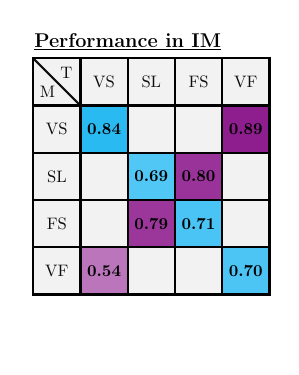
\begin{tikzpicture}[scale=0.6, every node/.style={transform shape}]
  % Label
  \node at (2., 11.85) {\large\underline{\textbf{Performance in IM}}};

  % Target/Masker
  \node at (0.7, 11.2) {T};
  \node at (0.3, 10.8) {M};
  \draw[thick] (0, 11.5) -- (1, 10.5);
  
  % Row labels
  \node at (1.5, 11.) {VS};
  \node at (2.5, 11.) {SL};
  \node at (3.5, 11.) {FS};
  \node at (4.5, 11.) {VF};
  % Column labels
  \node at (0.5, 10.) {VS};
  \node at (0.5, 9.) {SL};
  \node at (0.5, 8.) {FS};
  \node at (0.5, 7.) {VF};
  
  % Row 1 (top)
  \draw[thick, draw=black, fill=gray, fill opacity=0.1]
     (0, 10.5) -- (0, 11.5) -- (1, 11.5) -- (1, 10.5) -- cycle;
  \draw[thick, draw=black, fill=gray, fill opacity=0.1]
     (1, 10.5) -- (1, 11.5) -- (2, 11.5) -- (2, 10.5) -- cycle;
  \draw[thick, draw=black, fill=gray, fill opacity=0.1]
     (2, 10.5) -- (2, 11.5) -- (3, 11.5) -- (3, 10.5) -- cycle;
  \draw[thick, draw=black, fill=gray, fill opacity=0.1]
     (3, 10.5) -- (3, 11.5) -- (4, 11.5) -- (4, 10.5) -- cycle;
  \draw[thick, draw=black, fill=gray, fill opacity=0.1]
     (4, 10.5) -- (4, 11.5) -- (5, 11.5) -- (5, 10.5) -- cycle;
  % Row 2
  \draw[thick, draw=black, fill=gray, fill opacity=0.1]
     (0, 9.5) -- (0, 10.5) -- (1, 10.5) -- (1, 9.5) -- cycle;
  \draw[thick, draw=black, fill=cyan, fill opacity=0.8375]
     (1, 9.5) -- (1, 10.5) -- (2, 10.5) -- (2, 9.5) -- cycle;
  \node at (1.5, 10.) {\textbf{0.84}};
  \draw[thick, draw=black, fill=gray, fill opacity=0.1]
     (2, 9.5) -- (2, 10.5) -- (3, 10.5) -- (3, 9.5) -- cycle;
  \draw[thick, draw=black, fill=gray, fill opacity=0.1]
     (3, 9.5) -- (3, 10.5) -- (4, 10.5) -- (4, 9.5) -- cycle;
  \draw[thick, draw=black, fill=violet, fill opacity=0.8875]
     (4, 9.5) -- (4, 10.5) -- (5, 10.5) -- (5, 9.5) -- cycle;
  \node at (4.5, 10.) {\textbf{0.89}};
  % Row 3
  \draw[thick, draw=black, fill=gray, fill opacity=0.1]
     (0, 8.5) -- (0, 9.5) -- (1, 9.5) -- (1, 8.5) -- cycle;
  \draw[thick, draw=black, fill=gray, fill opacity=0.1]
     (1, 8.5) -- (1, 9.5) -- (2, 9.5) -- (2, 8.5) -- cycle;
  \draw[thick, draw=black, fill=cyan, fill opacity=0.6875]
     (2, 8.5) -- (2, 9.5) -- (3, 9.5) -- (3, 8.5) -- cycle;
  \node at (2.5, 9.) {\textbf{0.69}};
  \draw[thick, draw=black, fill=violet, fill opacity=0.8]
     (3, 8.5) -- (3, 9.5) -- (4, 9.5) -- (4, 8.5) -- cycle;
  \node at (3.5, 9.) {\textbf{0.80}};
  \draw[thick, draw=black, fill=gray, fill opacity=0.1]
     (4, 8.5) -- (4, 9.5) -- (5, 9.5) -- (5, 8.5) -- cycle;
  % Row 4
  \draw[thick, draw=black, fill=gray, fill opacity=0.1]
     (0, 7.5) -- (0, 8.5) -- (1, 8.5) -- (1, 7.5) -- cycle;
  \draw[thick, draw=black, fill=gray, fill opacity=0.1]
     (1, 7.5) -- (1, 8.5) -- (2, 8.5) -- (2, 7.5) -- cycle;
  \draw[thick, draw=black, fill=violet, fill opacity=0.7875]
     (2, 7.5) -- (2, 8.5) -- (3, 8.5) -- (3, 7.5) -- cycle;
  \node at (2.5, 8.) {\textbf{0.79}};
  \draw[thick, draw=black, fill=cyan, fill opacity=0.7125]
     (3, 7.5) -- (3, 8.5) -- (4, 8.5) -- (4, 7.5) -- cycle;
  \node at (3.5, 8.) {\textbf{0.71}};
  \draw[thick, draw=black, fill=gray, fill opacity=0.1]
     (4, 7.5) -- (4, 8.5) -- (5, 8.5) -- (5, 7.5) -- cycle;
  % Row 5 (bottom)
  \draw[thick, draw=black, fill=gray, fill opacity=0.1]
     (0, 6.5) -- (0, 7.5) -- (1, 7.5) -- (1, 6.5) -- cycle;
  \draw[thick, draw=black, fill=violet, fill opacity=0.5375]
     (1, 6.5) -- (1, 7.5) -- (2, 7.5) -- (2, 6.5) -- cycle;
  \node at (1.5, 7.) {\textbf{0.54}};
  \draw[thick, draw=black, fill=gray, fill opacity=0.1]
     (2, 6.5) -- (2, 7.5) -- (3, 7.5) -- (3, 6.5) -- cycle;
  \draw[thick, draw=black, fill=gray, fill opacity=0.1]
     (3, 6.5) -- (3, 7.5) -- (4, 7.5) -- (4, 6.5) -- cycle;
  \draw[thick, draw=black, fill=cyan, fill opacity=0.7]
     (4, 6.5) -- (4, 7.5) -- (5, 7.5) -- (5, 6.5) -- cycle;
  \node at (4.5, 7.) {\textbf{0.70}};
  
  % Invisible node to force the matrix up
  \node at (0, 5.5) {};
\end{tikzpicture}



\end{tabular}

%%%%%%%%%%%%%%%%%%%%%%%%%%%%%%%%%%%%%%%%%%%%%%%%%%
%%%%%%%%%%%%%%%%%%%%%%%%%%%%%%%%%%%%%%%%%%%%%%%%%%
\end{document}
